\begin{figure}[H] \centering 
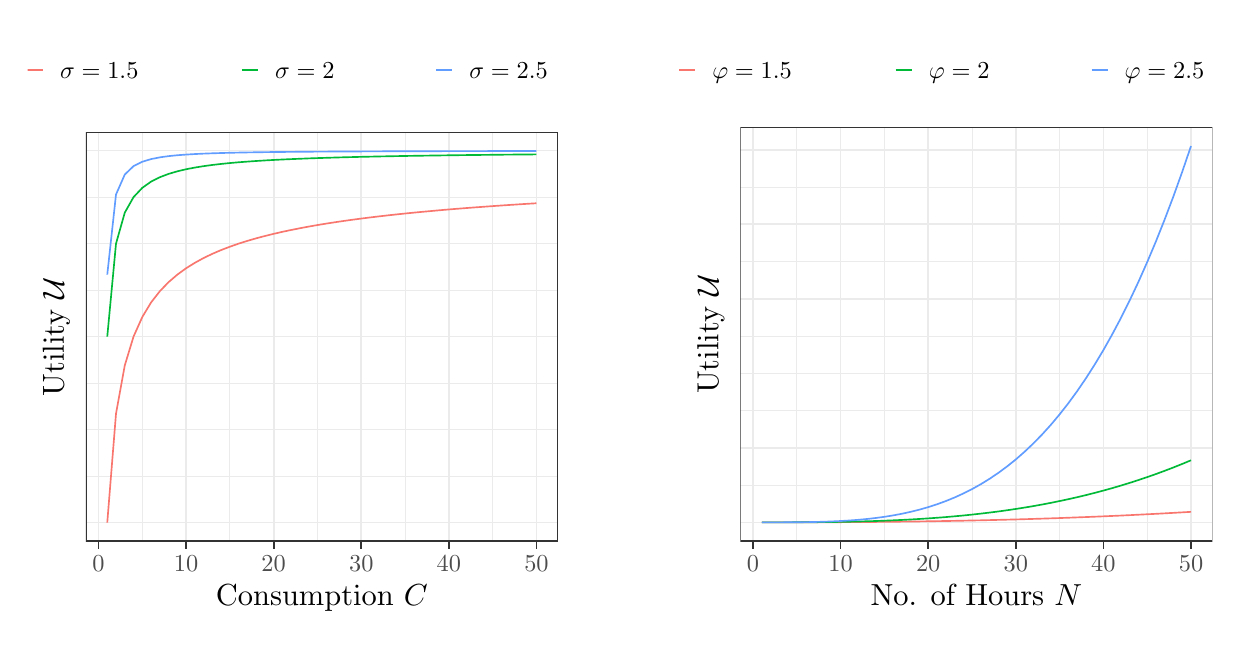
\begin{tikzpicture}[x=1pt,y=1pt]
\definecolor{fillColor}{RGB}{255,255,255}
\path[use as bounding box,fill=fillColor,fill opacity=0.00] (0,0) rectangle (433.62,216.81);
\begin{scope}
\path[clip] (  0.00,  0.00) rectangle (197.10,216.81);
\definecolor{drawColor}{RGB}{255,255,255}
\definecolor{fillColor}{RGB}{255,255,255}

\path[draw=drawColor,line width= 0.6pt,line join=round,line cap=round,fill=fillColor] (  0.00,  0.00) rectangle (197.10,216.81);
\end{scope}
\begin{scope}
\path[clip] ( 21.01, 31.25) rectangle (191.60,178.95);
\definecolor{fillColor}{RGB}{255,255,255}

\path[fill=fillColor] ( 21.01, 31.25) rectangle (191.60,178.95);
\definecolor{drawColor}{gray}{0.92}

\path[draw=drawColor,line width= 0.3pt,line join=round] ( 21.01, 54.77) --
	(191.60, 54.77);

\path[draw=drawColor,line width= 0.3pt,line join=round] ( 21.01, 88.37) --
	(191.60, 88.37);

\path[draw=drawColor,line width= 0.3pt,line join=round] ( 21.01,121.97) --
	(191.60,121.97);

\path[draw=drawColor,line width= 0.3pt,line join=round] ( 21.01,155.57) --
	(191.60,155.57);

\path[draw=drawColor,line width= 0.3pt,line join=round] ( 41.42, 31.25) --
	( 41.42,178.95);

\path[draw=drawColor,line width= 0.3pt,line join=round] ( 73.07, 31.25) --
	( 73.07,178.95);

\path[draw=drawColor,line width= 0.3pt,line join=round] (104.72, 31.25) --
	(104.72,178.95);

\path[draw=drawColor,line width= 0.3pt,line join=round] (136.37, 31.25) --
	(136.37,178.95);

\path[draw=drawColor,line width= 0.3pt,line join=round] (168.02, 31.25) --
	(168.02,178.95);

\path[draw=drawColor,line width= 0.6pt,line join=round] ( 21.01, 37.97) --
	(191.60, 37.97);

\path[draw=drawColor,line width= 0.6pt,line join=round] ( 21.01, 71.57) --
	(191.60, 71.57);

\path[draw=drawColor,line width= 0.6pt,line join=round] ( 21.01,105.17) --
	(191.60,105.17);

\path[draw=drawColor,line width= 0.6pt,line join=round] ( 21.01,138.77) --
	(191.60,138.77);

\path[draw=drawColor,line width= 0.6pt,line join=round] ( 21.01,172.37) --
	(191.60,172.37);

\path[draw=drawColor,line width= 0.6pt,line join=round] ( 25.59, 31.25) --
	( 25.59,178.95);

\path[draw=drawColor,line width= 0.6pt,line join=round] ( 57.24, 31.25) --
	( 57.24,178.95);

\path[draw=drawColor,line width= 0.6pt,line join=round] ( 88.89, 31.25) --
	( 88.89,178.95);

\path[draw=drawColor,line width= 0.6pt,line join=round] (120.55, 31.25) --
	(120.55,178.95);

\path[draw=drawColor,line width= 0.6pt,line join=round] (152.20, 31.25) --
	(152.20,178.95);

\path[draw=drawColor,line width= 0.6pt,line join=round] (183.85, 31.25) --
	(183.85,178.95);
\definecolor{drawColor}{RGB}{248,118,109}

\path[draw=drawColor,line width= 0.6pt,line join=round] ( 28.76, 37.97) --
	( 31.92, 77.33) --
	( 35.09, 94.77) --
	( 38.25,105.17) --
	( 41.42,112.26) --
	( 44.58,117.50) --
	( 47.75,121.57) --
	( 50.91,124.85) --
	( 54.08,127.57) --
	( 57.24,129.87) --
	( 60.41,131.84) --
	( 63.57,133.57) --
	( 66.74,135.09) --
	( 69.90,136.45) --
	( 73.07,137.66) --
	( 76.23,138.77) --
	( 79.40,139.77) --
	( 82.56,140.69) --
	( 85.73,141.53) --
	( 88.89,142.31) --
	( 92.06,143.04) --
	( 95.22,143.71) --
	( 98.39,144.34) --
	(101.55,144.93) --
	(104.72,145.49) --
	(107.89,146.01) --
	(111.05,146.50) --
	(114.22,146.97) --
	(117.38,147.41) --
	(120.55,147.83) --
	(123.71,148.23) --
	(126.88,148.61) --
	(130.04,148.97) --
	(133.21,149.32) --
	(136.37,149.65) --
	(139.54,149.97) --
	(142.70,150.27) --
	(145.87,150.56) --
	(149.03,150.85) --
	(152.20,151.12) --
	(155.36,151.38) --
	(158.53,151.63) --
	(161.69,151.87) --
	(164.86,152.10) --
	(168.02,152.33) --
	(171.19,152.55) --
	(174.35,152.76) --
	(177.52,152.97) --
	(180.68,153.17) --
	(183.85,153.36);
\definecolor{drawColor}{RGB}{0,186,56}

\path[draw=drawColor,line width= 0.6pt,line join=round] ( 28.76,105.17) --
	( 31.92,138.77) --
	( 35.09,149.97) --
	( 38.25,155.57) --
	( 41.42,158.93) --
	( 44.58,161.17) --
	( 47.75,162.77) --
	( 50.91,163.97) --
	( 54.08,164.90) --
	( 57.24,165.65) --
	( 60.41,166.26) --
	( 63.57,166.77) --
	( 66.74,167.20) --
	( 69.90,167.57) --
	( 73.07,167.89) --
	( 76.23,168.17) --
	( 79.40,168.41) --
	( 82.56,168.63) --
	( 85.73,168.83) --
	( 88.89,169.01) --
	( 92.06,169.17) --
	( 95.22,169.31) --
	( 98.39,169.44) --
	(101.55,169.57) --
	(104.72,169.68) --
	(107.89,169.78) --
	(111.05,169.88) --
	(114.22,169.97) --
	(117.38,170.05) --
	(120.55,170.13) --
	(123.71,170.20) --
	(126.88,170.27) --
	(130.04,170.33) --
	(133.21,170.39) --
	(136.37,170.45) --
	(139.54,170.50) --
	(142.70,170.55) --
	(145.87,170.60) --
	(149.03,170.64) --
	(152.20,170.69) --
	(155.36,170.73) --
	(158.53,170.77) --
	(161.69,170.80) --
	(164.86,170.84) --
	(168.02,170.87) --
	(171.19,170.91) --
	(174.35,170.94) --
	(177.52,170.97) --
	(180.68,170.99) --
	(183.85,171.02);
\definecolor{drawColor}{RGB}{97,156,255}

\path[draw=drawColor,line width= 0.6pt,line join=round] ( 28.76,127.57) --
	( 31.92,156.53) --
	( 35.09,163.74) --
	( 38.25,166.77) --
	( 41.42,168.36) --
	( 44.58,169.32) --
	( 47.75,169.95) --
	( 50.91,170.39) --
	( 54.08,170.71) --
	( 57.24,170.95) --
	( 60.41,171.14) --
	( 63.57,171.29) --
	( 66.74,171.41) --
	( 69.90,171.51) --
	( 73.07,171.60) --
	( 76.23,171.67) --
	( 79.40,171.73) --
	( 82.56,171.78) --
	( 85.73,171.83) --
	( 88.89,171.87) --
	( 92.06,171.90) --
	( 95.22,171.93) --
	( 98.39,171.96) --
	(101.55,171.99) --
	(104.72,172.01) --
	(107.89,172.03) --
	(111.05,172.05) --
	(114.22,172.06) --
	(117.38,172.08) --
	(120.55,172.09) --
	(123.71,172.11) --
	(126.88,172.12) --
	(130.04,172.13) --
	(133.21,172.14) --
	(136.37,172.15) --
	(139.54,172.16) --
	(142.70,172.17) --
	(145.87,172.18) --
	(149.03,172.18) --
	(152.20,172.19) --
	(155.36,172.20) --
	(158.53,172.20) --
	(161.69,172.21) --
	(164.86,172.21) --
	(168.02,172.22) --
	(171.19,172.22) --
	(174.35,172.23) --
	(177.52,172.23) --
	(180.68,172.24) --
	(183.85,172.24);
\definecolor{drawColor}{gray}{0.20}

\path[draw=drawColor,line width= 0.6pt,line join=round,line cap=round] ( 21.01, 31.25) rectangle (191.60,178.95);
\end{scope}
\begin{scope}
\path[clip] (  0.00,  0.00) rectangle (433.62,216.81);
\definecolor{drawColor}{gray}{0.20}

\path[draw=drawColor,line width= 0.6pt,line join=round] ( 25.59, 28.50) --
	( 25.59, 31.25);

\path[draw=drawColor,line width= 0.6pt,line join=round] ( 57.24, 28.50) --
	( 57.24, 31.25);

\path[draw=drawColor,line width= 0.6pt,line join=round] ( 88.89, 28.50) --
	( 88.89, 31.25);

\path[draw=drawColor,line width= 0.6pt,line join=round] (120.55, 28.50) --
	(120.55, 31.25);

\path[draw=drawColor,line width= 0.6pt,line join=round] (152.20, 28.50) --
	(152.20, 31.25);

\path[draw=drawColor,line width= 0.6pt,line join=round] (183.85, 28.50) --
	(183.85, 31.25);
\end{scope}
\begin{scope}
\path[clip] (  0.00,  0.00) rectangle (433.62,216.81);
\definecolor{drawColor}{gray}{0.30}

\node[text=drawColor,anchor=base,inner sep=0pt, outer sep=0pt, scale=  0.88] at ( 25.59, 20.24) {0};

\node[text=drawColor,anchor=base,inner sep=0pt, outer sep=0pt, scale=  0.88] at ( 57.24, 20.24) {10};

\node[text=drawColor,anchor=base,inner sep=0pt, outer sep=0pt, scale=  0.88] at ( 88.89, 20.24) {20};

\node[text=drawColor,anchor=base,inner sep=0pt, outer sep=0pt, scale=  0.88] at (120.55, 20.24) {30};

\node[text=drawColor,anchor=base,inner sep=0pt, outer sep=0pt, scale=  0.88] at (152.20, 20.24) {40};

\node[text=drawColor,anchor=base,inner sep=0pt, outer sep=0pt, scale=  0.88] at (183.85, 20.24) {50};
\end{scope}
\begin{scope}
\path[clip] (  0.00,  0.00) rectangle (433.62,216.81);
\definecolor{drawColor}{RGB}{0,0,0}

\node[text=drawColor,anchor=base,inner sep=0pt, outer sep=0pt, scale=  1.10] at (106.30,  7.93) {Consumption $C$};
\end{scope}
\begin{scope}
\path[clip] (  0.00,  0.00) rectangle (433.62,216.81);
\definecolor{drawColor}{RGB}{0,0,0}

\node[text=drawColor,rotate= 90.00,anchor=base,inner sep=0pt, outer sep=0pt, scale=  1.10] at ( 13.08,105.10) {Utility $\mathcal{U}$};
\end{scope}
\begin{scope}
\path[clip] (  0.00,  0.00) rectangle (433.62,216.81);
\definecolor{fillColor}{RGB}{255,255,255}

\path[fill=fillColor] (-12.03,189.95) rectangle (224.63,211.31);
\end{scope}
\begin{scope}
\path[clip] (  0.00,  0.00) rectangle (433.62,216.81);
\definecolor{fillColor}{RGB}{255,255,255}

\path[fill=fillColor] ( -1.03,197.34) rectangle (  6.20,205.81);
\end{scope}
\begin{scope}
\path[clip] (  0.00,  0.00) rectangle (433.62,216.81);
\definecolor{drawColor}{RGB}{248,118,109}

\path[draw=drawColor,line width= 0.6pt,line join=round] ( -0.31,201.57) -- (  5.48,201.57);
\end{scope}
\begin{scope}
\path[clip] (  0.00,  0.00) rectangle (433.62,216.81);
\definecolor{fillColor}{RGB}{255,255,255}

\path[fill=fillColor] ( 76.70,197.34) rectangle ( 83.93,205.81);
\end{scope}
\begin{scope}
\path[clip] (  0.00,  0.00) rectangle (433.62,216.81);
\definecolor{drawColor}{RGB}{0,186,56}

\path[draw=drawColor,line width= 0.6pt,line join=round] ( 77.43,201.57) -- ( 83.21,201.57);
\end{scope}
\begin{scope}
\path[clip] (  0.00,  0.00) rectangle (433.62,216.81);
\definecolor{fillColor}{RGB}{255,255,255}

\path[fill=fillColor] (146.90,197.34) rectangle (154.13,205.81);
\end{scope}
\begin{scope}
\path[clip] (  0.00,  0.00) rectangle (433.62,216.81);
\definecolor{drawColor}{RGB}{97,156,255}

\path[draw=drawColor,line width= 0.6pt,line join=round] (147.62,201.57) -- (153.41,201.57);
\end{scope}
\begin{scope}
\path[clip] (  0.00,  0.00) rectangle (433.62,216.81);
\definecolor{drawColor}{RGB}{0,0,0}

\node[text=drawColor,anchor=base west,inner sep=0pt, outer sep=0pt, scale=  0.88] at ( 11.70,198.54) {$\sigma = 1.5$};
\end{scope}
\begin{scope}
\path[clip] (  0.00,  0.00) rectangle (433.62,216.81);
\definecolor{drawColor}{RGB}{0,0,0}

\node[text=drawColor,anchor=base west,inner sep=0pt, outer sep=0pt, scale=  0.88] at ( 89.43,198.54) {$\sigma = 2$};
\end{scope}
\begin{scope}
\path[clip] (  0.00,  0.00) rectangle (433.62,216.81);
\definecolor{drawColor}{RGB}{0,0,0}

\node[text=drawColor,anchor=base west,inner sep=0pt, outer sep=0pt, scale=  0.88] at (159.63,198.54) {$\sigma = 2.5$};
\end{scope}
\begin{scope}
\path[clip] (236.52,  0.00) rectangle (433.62,216.81);
\definecolor{drawColor}{RGB}{255,255,255}
\definecolor{fillColor}{RGB}{255,255,255}

\path[draw=drawColor,line width= 0.6pt,line join=round,line cap=round,fill=fillColor] (236.52,  0.00) rectangle (433.62,216.81);
\end{scope}
\begin{scope}
\path[clip] (257.53, 31.25) rectangle (428.12,180.84);
\definecolor{fillColor}{RGB}{255,255,255}

\path[fill=fillColor] (257.53, 31.25) rectangle (428.12,180.84);
\definecolor{drawColor}{gray}{0.92}

\path[draw=drawColor,line width= 0.3pt,line join=round] (257.53, 51.51) --
	(428.12, 51.51);

\path[draw=drawColor,line width= 0.3pt,line join=round] (257.53, 78.44) --
	(428.12, 78.44);

\path[draw=drawColor,line width= 0.3pt,line join=round] (257.53,105.36) --
	(428.12,105.36);

\path[draw=drawColor,line width= 0.3pt,line join=round] (257.53,132.28) --
	(428.12,132.28);

\path[draw=drawColor,line width= 0.3pt,line join=round] (257.53,159.21) --
	(428.12,159.21);

\path[draw=drawColor,line width= 0.3pt,line join=round] (277.94, 31.25) --
	(277.94,180.84);

\path[draw=drawColor,line width= 0.3pt,line join=round] (309.59, 31.25) --
	(309.59,180.84);

\path[draw=drawColor,line width= 0.3pt,line join=round] (341.24, 31.25) --
	(341.24,180.84);

\path[draw=drawColor,line width= 0.3pt,line join=round] (372.89, 31.25) --
	(372.89,180.84);

\path[draw=drawColor,line width= 0.3pt,line join=round] (404.54, 31.25) --
	(404.54,180.84);

\path[draw=drawColor,line width= 0.6pt,line join=round] (257.53, 38.05) --
	(428.12, 38.05);

\path[draw=drawColor,line width= 0.6pt,line join=round] (257.53, 64.98) --
	(428.12, 64.98);

\path[draw=drawColor,line width= 0.6pt,line join=round] (257.53, 91.90) --
	(428.12, 91.90);

\path[draw=drawColor,line width= 0.6pt,line join=round] (257.53,118.82) --
	(428.12,118.82);

\path[draw=drawColor,line width= 0.6pt,line join=round] (257.53,145.75) --
	(428.12,145.75);

\path[draw=drawColor,line width= 0.6pt,line join=round] (257.53,172.67) --
	(428.12,172.67);

\path[draw=drawColor,line width= 0.6pt,line join=round] (262.11, 31.25) --
	(262.11,180.84);

\path[draw=drawColor,line width= 0.6pt,line join=round] (293.76, 31.25) --
	(293.76,180.84);

\path[draw=drawColor,line width= 0.6pt,line join=round] (325.41, 31.25) --
	(325.41,180.84);

\path[draw=drawColor,line width= 0.6pt,line join=round] (357.07, 31.25) --
	(357.07,180.84);

\path[draw=drawColor,line width= 0.6pt,line join=round] (388.72, 31.25) --
	(388.72,180.84);

\path[draw=drawColor,line width= 0.6pt,line join=round] (420.37, 31.25) --
	(420.37,180.84);
\definecolor{drawColor}{RGB}{248,118,109}

\path[draw=drawColor,line width= 0.6pt,line join=round] (265.28, 38.05) --
	(268.44, 38.05) --
	(271.61, 38.06) --
	(274.77, 38.06) --
	(277.94, 38.06) --
	(281.10, 38.07) --
	(284.27, 38.08) --
	(287.43, 38.09) --
	(290.60, 38.10) --
	(293.76, 38.12) --
	(296.93, 38.14) --
	(300.09, 38.16) --
	(303.26, 38.18) --
	(306.42, 38.21) --
	(309.59, 38.24) --
	(312.75, 38.27) --
	(315.92, 38.31) --
	(319.08, 38.35) --
	(322.25, 38.39) --
	(325.41, 38.44) --
	(328.58, 38.49) --
	(331.74, 38.54) --
	(334.91, 38.60) --
	(338.07, 38.66) --
	(341.24, 38.73) --
	(344.41, 38.79) --
	(347.57, 38.87) --
	(350.74, 38.95) --
	(353.90, 39.03) --
	(357.07, 39.11) --
	(360.23, 39.20) --
	(363.40, 39.30) --
	(366.56, 39.40) --
	(369.73, 39.50) --
	(372.89, 39.61) --
	(376.06, 39.73) --
	(379.22, 39.85) --
	(382.39, 39.97) --
	(385.55, 40.10) --
	(388.72, 40.23) --
	(391.88, 40.37) --
	(395.05, 40.51) --
	(398.21, 40.66) --
	(401.38, 40.82) --
	(404.54, 40.98) --
	(407.71, 41.14) --
	(410.87, 41.31) --
	(414.04, 41.49) --
	(417.20, 41.67) --
	(420.37, 41.86);
\definecolor{drawColor}{RGB}{0,186,56}

\path[draw=drawColor,line width= 0.6pt,line join=round] (265.28, 38.05) --
	(268.44, 38.05) --
	(271.61, 38.06) --
	(274.77, 38.06) --
	(277.94, 38.07) --
	(281.10, 38.09) --
	(284.27, 38.11) --
	(287.43, 38.14) --
	(290.60, 38.18) --
	(293.76, 38.23) --
	(296.93, 38.29) --
	(300.09, 38.36) --
	(303.26, 38.45) --
	(306.42, 38.54) --
	(309.59, 38.66) --
	(312.75, 38.79) --
	(315.92, 38.93) --
	(319.08, 39.10) --
	(322.25, 39.28) --
	(325.41, 39.49) --
	(328.58, 39.71) --
	(331.74, 39.96) --
	(334.91, 40.24) --
	(338.07, 40.53) --
	(341.24, 40.86) --
	(344.41, 41.21) --
	(347.57, 41.59) --
	(350.74, 41.99) --
	(353.90, 42.43) --
	(357.07, 42.90) --
	(360.23, 43.40) --
	(363.40, 43.93) --
	(366.56, 44.50) --
	(369.73, 45.11) --
	(372.89, 45.75) --
	(376.06, 46.43) --
	(379.22, 47.14) --
	(382.39, 47.90) --
	(385.55, 48.70) --
	(388.72, 49.54) --
	(391.88, 50.42) --
	(395.05, 51.35) --
	(398.21, 52.32) --
	(401.38, 53.34) --
	(404.54, 54.41) --
	(407.71, 55.52) --
	(410.87, 56.69) --
	(414.04, 57.90) --
	(417.20, 59.17) --
	(420.37, 60.49);
\definecolor{drawColor}{RGB}{97,156,255}

\path[draw=drawColor,line width= 0.6pt,line join=round] (265.28, 38.05) --
	(268.44, 38.05) --
	(271.61, 38.06) --
	(274.77, 38.07) --
	(277.94, 38.10) --
	(281.10, 38.13) --
	(284.27, 38.19) --
	(287.43, 38.28) --
	(290.60, 38.39) --
	(293.76, 38.54) --
	(296.93, 38.73) --
	(300.09, 38.97) --
	(303.26, 39.27) --
	(306.42, 39.63) --
	(309.59, 40.06) --
	(312.75, 40.57) --
	(315.92, 41.17) --
	(319.08, 41.86) --
	(322.25, 42.65) --
	(325.41, 43.56) --
	(328.58, 44.58) --
	(331.74, 45.74) --
	(334.91, 47.03) --
	(338.07, 48.47) --
	(341.24, 50.07) --
	(344.41, 51.84) --
	(347.57, 53.79) --
	(350.74, 55.92) --
	(353.90, 58.26) --
	(357.07, 60.80) --
	(360.23, 63.57) --
	(363.40, 66.57) --
	(366.56, 69.81) --
	(369.73, 73.31) --
	(372.89, 77.08) --
	(376.06, 81.12) --
	(379.22, 85.45) --
	(382.39, 90.09) --
	(385.55, 95.05) --
	(388.72,100.33) --
	(391.88,105.95) --
	(395.05,111.92) --
	(398.21,118.26) --
	(401.38,124.98) --
	(404.54,132.10) --
	(407.71,139.62) --
	(410.87,147.56) --
	(414.04,155.93) --
	(417.20,164.75) --
	(420.37,174.04);
\definecolor{drawColor}{gray}{0.20}

\path[draw=drawColor,line width= 0.6pt,line join=round,line cap=round] (257.53, 31.25) rectangle (428.12,180.84);
\end{scope}
\begin{scope}
\path[clip] (  0.00,  0.00) rectangle (433.62,216.81);
\definecolor{drawColor}{gray}{0.20}

\path[draw=drawColor,line width= 0.6pt,line join=round] (262.11, 28.50) --
	(262.11, 31.25);

\path[draw=drawColor,line width= 0.6pt,line join=round] (293.76, 28.50) --
	(293.76, 31.25);

\path[draw=drawColor,line width= 0.6pt,line join=round] (325.41, 28.50) --
	(325.41, 31.25);

\path[draw=drawColor,line width= 0.6pt,line join=round] (357.07, 28.50) --
	(357.07, 31.25);

\path[draw=drawColor,line width= 0.6pt,line join=round] (388.72, 28.50) --
	(388.72, 31.25);

\path[draw=drawColor,line width= 0.6pt,line join=round] (420.37, 28.50) --
	(420.37, 31.25);
\end{scope}
\begin{scope}
\path[clip] (  0.00,  0.00) rectangle (433.62,216.81);
\definecolor{drawColor}{gray}{0.30}

\node[text=drawColor,anchor=base,inner sep=0pt, outer sep=0pt, scale=  0.88] at (262.11, 20.24) {0};

\node[text=drawColor,anchor=base,inner sep=0pt, outer sep=0pt, scale=  0.88] at (293.76, 20.24) {10};

\node[text=drawColor,anchor=base,inner sep=0pt, outer sep=0pt, scale=  0.88] at (325.41, 20.24) {20};

\node[text=drawColor,anchor=base,inner sep=0pt, outer sep=0pt, scale=  0.88] at (357.07, 20.24) {30};

\node[text=drawColor,anchor=base,inner sep=0pt, outer sep=0pt, scale=  0.88] at (388.72, 20.24) {40};

\node[text=drawColor,anchor=base,inner sep=0pt, outer sep=0pt, scale=  0.88] at (420.37, 20.24) {50};
\end{scope}
\begin{scope}
\path[clip] (  0.00,  0.00) rectangle (433.62,216.81);
\definecolor{drawColor}{RGB}{0,0,0}

\node[text=drawColor,anchor=base,inner sep=0pt, outer sep=0pt, scale=  1.10] at (342.82,  7.93) {No. of Hours $N$};
\end{scope}
\begin{scope}
\path[clip] (  0.00,  0.00) rectangle (433.62,216.81);
\definecolor{drawColor}{RGB}{0,0,0}

\node[text=drawColor,rotate= 90.00,anchor=base,inner sep=0pt, outer sep=0pt, scale=  1.10] at (249.60,106.04) {Utility $\mathcal{U}$};
\end{scope}
\begin{scope}
\path[clip] (  0.00,  0.00) rectangle (433.62,216.81);
\definecolor{fillColor}{RGB}{255,255,255}

\path[fill=fillColor] (223.66,191.84) rectangle (461.98,211.31);
\end{scope}
\begin{scope}
\path[clip] (  0.00,  0.00) rectangle (433.62,216.81);
\definecolor{fillColor}{RGB}{255,255,255}

\path[fill=fillColor] (234.66,197.34) rectangle (241.89,205.81);
\end{scope}
\begin{scope}
\path[clip] (  0.00,  0.00) rectangle (433.62,216.81);
\definecolor{drawColor}{RGB}{248,118,109}

\path[draw=drawColor,line width= 0.6pt,line join=round] (235.39,201.57) -- (241.17,201.57);
\end{scope}
\begin{scope}
\path[clip] (  0.00,  0.00) rectangle (433.62,216.81);
\definecolor{fillColor}{RGB}{255,255,255}

\path[fill=fillColor] (312.95,197.34) rectangle (320.17,205.81);
\end{scope}
\begin{scope}
\path[clip] (  0.00,  0.00) rectangle (433.62,216.81);
\definecolor{drawColor}{RGB}{0,186,56}

\path[draw=drawColor,line width= 0.6pt,line join=round] (313.67,201.57) -- (319.45,201.57);
\end{scope}
\begin{scope}
\path[clip] (  0.00,  0.00) rectangle (433.62,216.81);
\definecolor{fillColor}{RGB}{255,255,255}

\path[fill=fillColor] (383.70,197.34) rectangle (390.92,205.81);
\end{scope}
\begin{scope}
\path[clip] (  0.00,  0.00) rectangle (433.62,216.81);
\definecolor{drawColor}{RGB}{97,156,255}

\path[draw=drawColor,line width= 0.6pt,line join=round] (384.42,201.57) -- (390.20,201.57);
\end{scope}
\begin{scope}
\path[clip] (  0.00,  0.00) rectangle (433.62,216.81);
\definecolor{drawColor}{RGB}{0,0,0}

\node[text=drawColor,anchor=base west,inner sep=0pt, outer sep=0pt, scale=  0.88] at (247.39,198.54) {$\varphi = 1.5$};
\end{scope}
\begin{scope}
\path[clip] (  0.00,  0.00) rectangle (433.62,216.81);
\definecolor{drawColor}{RGB}{0,0,0}

\node[text=drawColor,anchor=base west,inner sep=0pt, outer sep=0pt, scale=  0.88] at (325.67,198.54) {$\varphi = 2$};
\end{scope}
\begin{scope}
\path[clip] (  0.00,  0.00) rectangle (433.62,216.81);
\definecolor{drawColor}{RGB}{0,0,0}

\node[text=drawColor,anchor=base west,inner sep=0pt, outer sep=0pt, scale=  0.88] at (396.42,198.54) {$\varphi = 2.5$};
\end{scope}
\end{tikzpicture}\end{figure}